\chapter{O solo vivo}\label{ch:b2:living-soil}

O último livro de Charles Darwin, publicado um ano antes de sua morte,
tratava das minhocas. Ele tinha colocado um marcador de giz num campo
perto de sua casa em 1842 e o desenterrou em 1871: estava a dezoito
centímetros de profundidade, enterrado pelos excrementos que as minhocas
tinham trazido à superfície num ritmo que ele mediu, pesou e multiplicou
--- dez toneladas de \omterm{def:b2:living-soil:soil}{solo} por acre por ano passando por seus corpos, de
modo que ``toda a terra vegetal superficial de qualquer extensão desse
tipo passou, e voltará a passar, a cada poucos anos, pelo corpo das
minhocas''. O \omterm{def:b2:living-soil:soil}{solo}, em outras palavras, não é um substrato sobre o qual
os seres vivos se apoiam, mas algo que os seres vivos fazem. Este
capítulo trata dessa fabricação: como a rocha se torna \omterm{def:b2:living-soil:soil}{solo} e com que
lentidão, quem vive nele e em que números, como a matéria morta é
desmontada e o que resta, como as raízes das plantas negociam com
fungos e bactérias aquilo que não conseguem obter sozinhas, e com que
rapidez um \omterm{def:b2:living-soil:soil}{solo} que levou dez mil anos para se formar pode ser perdido.

\section{O que é o solo}

\begin{definition}[O solo e seus horizontes]\label{def:b2:living-soil:soil}
\index{solo}\index{horizonte do solo}\index{húmus}\index{intemperismo}\index{pedogênese}
O \emph{solo} é a camada de matéria mineral intemperizada, matéria
orgânica, água, ar e organismos que recobre as terras emersas e sustenta
as plantas: cerca de metade de seu volume são poros, cheios de água ou
de ar em proporções variáveis, e a metade sólida são grãos minerais ---
areia (\qtyrange{0.05}{2}{mm}), silte (\qtyrange{2}{50}{\micro m}) e
argila (menos de \qty{2}{\micro m}), cujas proporções dão a
\emph{textura} ---, com alguns por cento de matéria orgânica que
governa a maior parte de suas propriedades. Um perfil de solo mostra
\emph{horizontes}: o horizonte \emph{O}, de serapilheira e matéria
orgânica parcialmente decomposta, na superfície; o horizonte \emph{A},
escuro, de solo mineral misturado com \emph{húmus}, o resíduo estável,
escuro e coloidal da decomposição; o horizonte \emph{B}, abaixo, para o
qual a argila, o ferro e a matéria dissolvida são lavados e onde se
acumulam; o horizonte \emph{C}, de rocha-mãe intemperizada; e a rocha
matriz. Um solo é formado (\emph{pedogênese}) por cinco fatores ---
material de origem, clima, organismos, relevo e tempo --- e é formado
lentamente: o intemperismo produz da ordem de \qty{0.1}{mm} de
solo por ano, de modo que um metro de solo são dez mil anos de trabalho.
\end{definition}

\begin{omfigure}
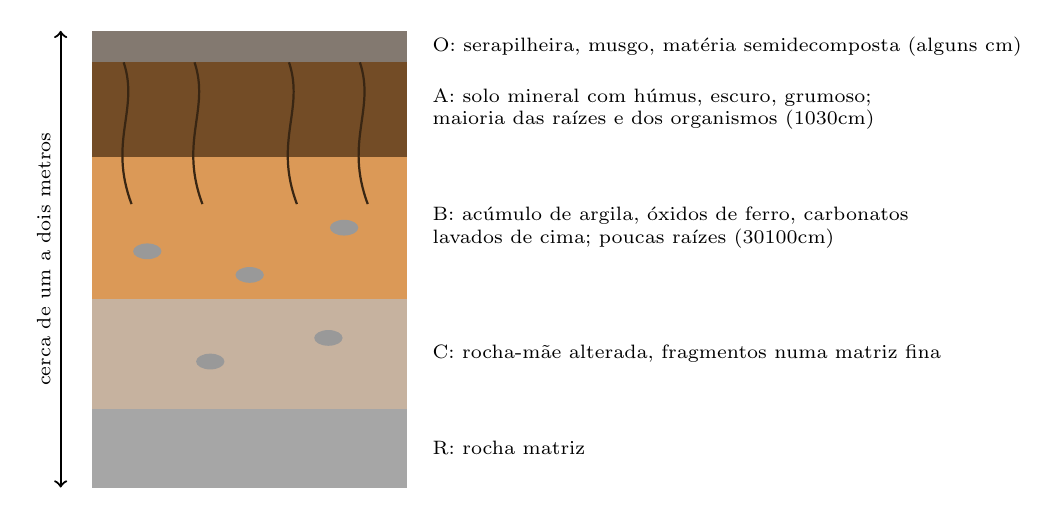
\begin{tikzpicture}[every node/.style={font=\scriptsize}]
  \fill[brown!25!black!60] (0,5.4) rectangle (4,5.8); \node[right] at (4.2,5.6) {O: serapilheira, musgo, matéria semidecomposta (alguns cm)};
  \fill[brown!60!black] (0,4.2) rectangle (4,5.4); \node[right, align=left] at (4.2,4.8) {A: solo mineral com húmus, escuro, grumoso;\\ maioria das raízes e dos organismos (\qtyrange{10}{30}{cm})};
  \fill[brown!70!orange!80] (0,2.4) rectangle (4,4.2); \node[right, align=left] at (4.2,3.3) {B: acúmulo de argila, óxidos de ferro, carbonatos\\ lavados de cima; poucas raízes (\qtyrange{30}{100}{cm})};
  \fill[gray!50!brown!60] (0,1.0) rectangle (4,2.4); \node[right, align=left] at (4.2,1.7) {C: rocha-mãe alterada, fragmentos numa matriz fina};
  \fill[gray!70] (0,0) rectangle (4,1.0); \node[right] at (4.2,0.5) {R: rocha matriz};
  \foreach \x in {0.4,1.3,2.5,3.4} \draw[brown!30!black, thick] (\x,5.4) .. controls (\x+0.2,4.8) and (\x-0.2,4.4) .. (\x+0.1,3.6);
  \foreach \x/\y in {0.7/3.0, 2.0/2.7, 3.2/3.3, 1.5/1.6, 3.0/1.9} \fill[gray!80] (\x,\y) ellipse (0.18 and 0.1);
  \draw[<->, thick] (-0.4,5.8) -- (-0.4,0) node[midway, left, rotate=90, anchor=south] {cerca de um a dois metros};
\end{tikzpicture}

{\small Um perfil de \omterm{def:b2:living-soil:soil}{solo}. A matéria orgânica entra pelo topo e é
consumida à medida que desce; a matéria mineral é liberada na base e
levada para cima pelas raízes e pelos animais; a matéria dissolvida
desce com a água e é retida no horizonte B.}
\end{omfigure}

\begin{proposition}[Por que a argila e o húmus importam]\label{prop:b2:living-soil:cec}
\index{capacidade de troca catiônica}\index{argila}\index{estrutura do solo}\index{capacidade de campo}
As partículas de argila e o \omterm{def:b2:living-soil:soil}{húmus} têm cargas negativas em sua superfície
e retêm, por atração eletrostática, uma reserva de cátions trocáveis ---
$\mathrm{Ca^{2+}}$, $\mathrm{Mg^{2+}}$, $\mathrm{K^{+}}$, $\mathrm{NH_4^{+}}$ --- dos quais
as raízes das plantas se servem trocando-os por $\mathrm{H^{+}}$. Essa
\emph{\omterm{prop:b2:living-soil:cec}{capacidade de troca catiônica}} é o banco de nutrientes do \omterm{def:b2:living-soil:soil}{solo};
uma areia quase não a tem (alguns centimols de carga por quilograma),
um franco-argiloso rico em \omterm{def:b2:living-soil:soil}{húmus} tem cinquenta vezes mais, e a
fertilidade dos dois difere na mesma proporção. As mesmas superfícies
retêm a água: um \omterm{def:b2:living-soil:soil}{solo} arenoso drena em um dia até uma \emph{\omterm{prop:b2:living-soil:cec}{capacidade
de campo}} de um décimo de seu volume, um \omterm{def:b2:living-soil:soil}{solo} franco retém um terço, e a
diferença é o que uma cultura tem à disposição entre duas chuvas. E o
\omterm{def:b2:living-soil:soil}{húmus}, junto com as hifas dos fungos, os exsudatos das raízes e o muco
das minhocas, cola os grãos minerais em \emph{agregados}, a estrutura
grumosa cujos poros deixam passar o ar, a água e as raízes --- a
propriedade que distingue um \omterm{def:b2:living-soil:soil}{solo} de um sedimento e que é destruída em
primeiro lugar pela aração e pela compactação.
\end{proposition}

\section{Quem vive lá}

\begin{proposition}[A comunidade do solo]\label{prop:b2:living-soil:community}
\index{teia alimentar do solo}\index{detritívoro}\index{minhoca}\index{biomassa do solo}
Um grama de camada superficial fértil contém cerca de $10^{9}$ células
bacterianas de umas dez mil espécies, cem metros de hifas de fungos, $10^{4}$
\omterm{def:b2:unicellular-diversity:protist}{protistas}, algumas dezenas de nematoides e um punhado de ácaros e
colêmbolos; um metro quadrado abriga algumas centenas de minhocas e,
abaixo dos animais visíveis, uma massa viva de várias toneladas por
hectare --- comparável ao gado que o mesmo hectare poderia sustentar. A
comunidade é uma \emph{teia alimentar detrítica}: as bactérias e os
fungos (os \emph{decompositores}) comem a matéria morta e são comidos
pelos \omterm{def:b2:unicellular-diversity:protist}{protistas} e pelos nematoides (os pastadores microbianos), que são
comidos pelos ácaros e pelos nematoides predadores, que alimentam
centopeias e besouros; os \emph{detritívoros} --- minhocas, diplópodes,
tatuzinhos, cupins, colêmbolos --- comem a própria serapilheira com os
micróbios que ela contém, fragmentando-a mil vezes e multiplicando a
superfície que os micróbios atacam. Os pastadores importam além de seu
número: ao comer bactérias, eles liberam na forma de amônio o nitrogênio
preso nas células bacterianas, e um \omterm{def:b2:living-soil:soil}{solo} com \omterm{def:b2:unicellular-diversity:protist}{protistas} e nematoides
mineraliza o nitrogênio mais depressa que um \omterm{def:b2:living-soil:soil}{solo} só com bactérias. As
minhocas são as \emph{engenheiras do ecossistema}: suas galerias são os
macroporos do \omterm{def:b2:living-soil:soil}{solo}, seus excrementos são os agregados mais ricos, e as
minhocas de uma pastagem fazem passar por seu intestino algumas
toneladas de \omterm{def:b2:living-soil:soil}{solo} por hectare a cada ano, como Darwin mediu.
\end{proposition}

\begin{omfigure}
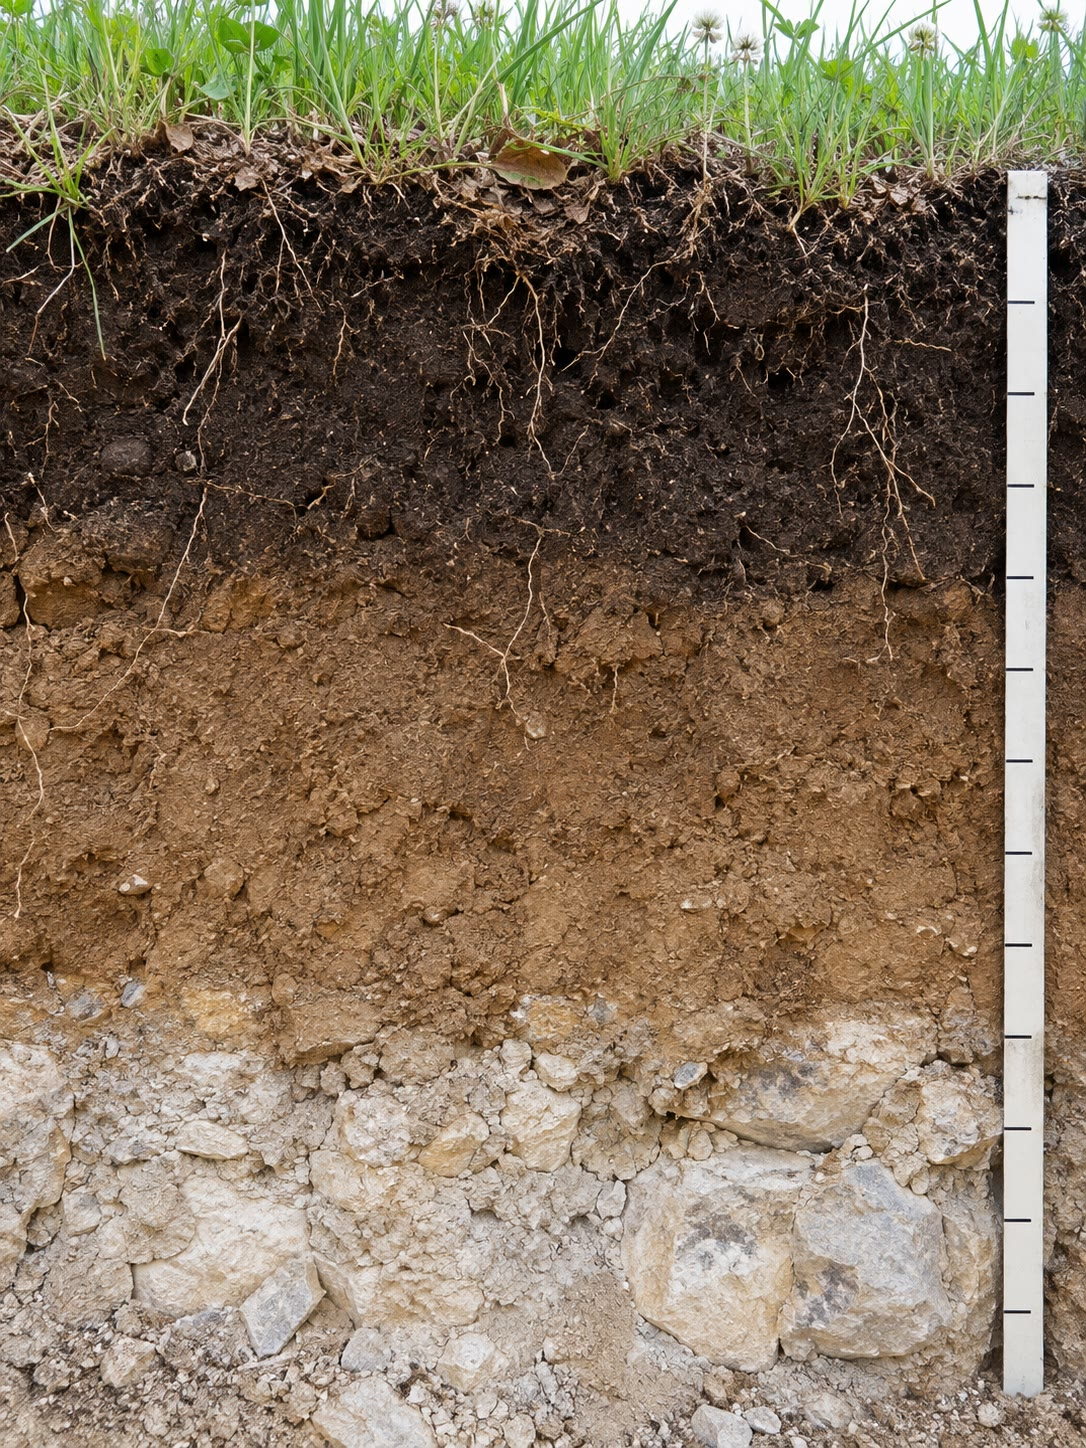
\includegraphics[width=0.21\linewidth]{images/book4/ai/b4-26-soil-profile.jpg}\hspace{0.025\linewidth}
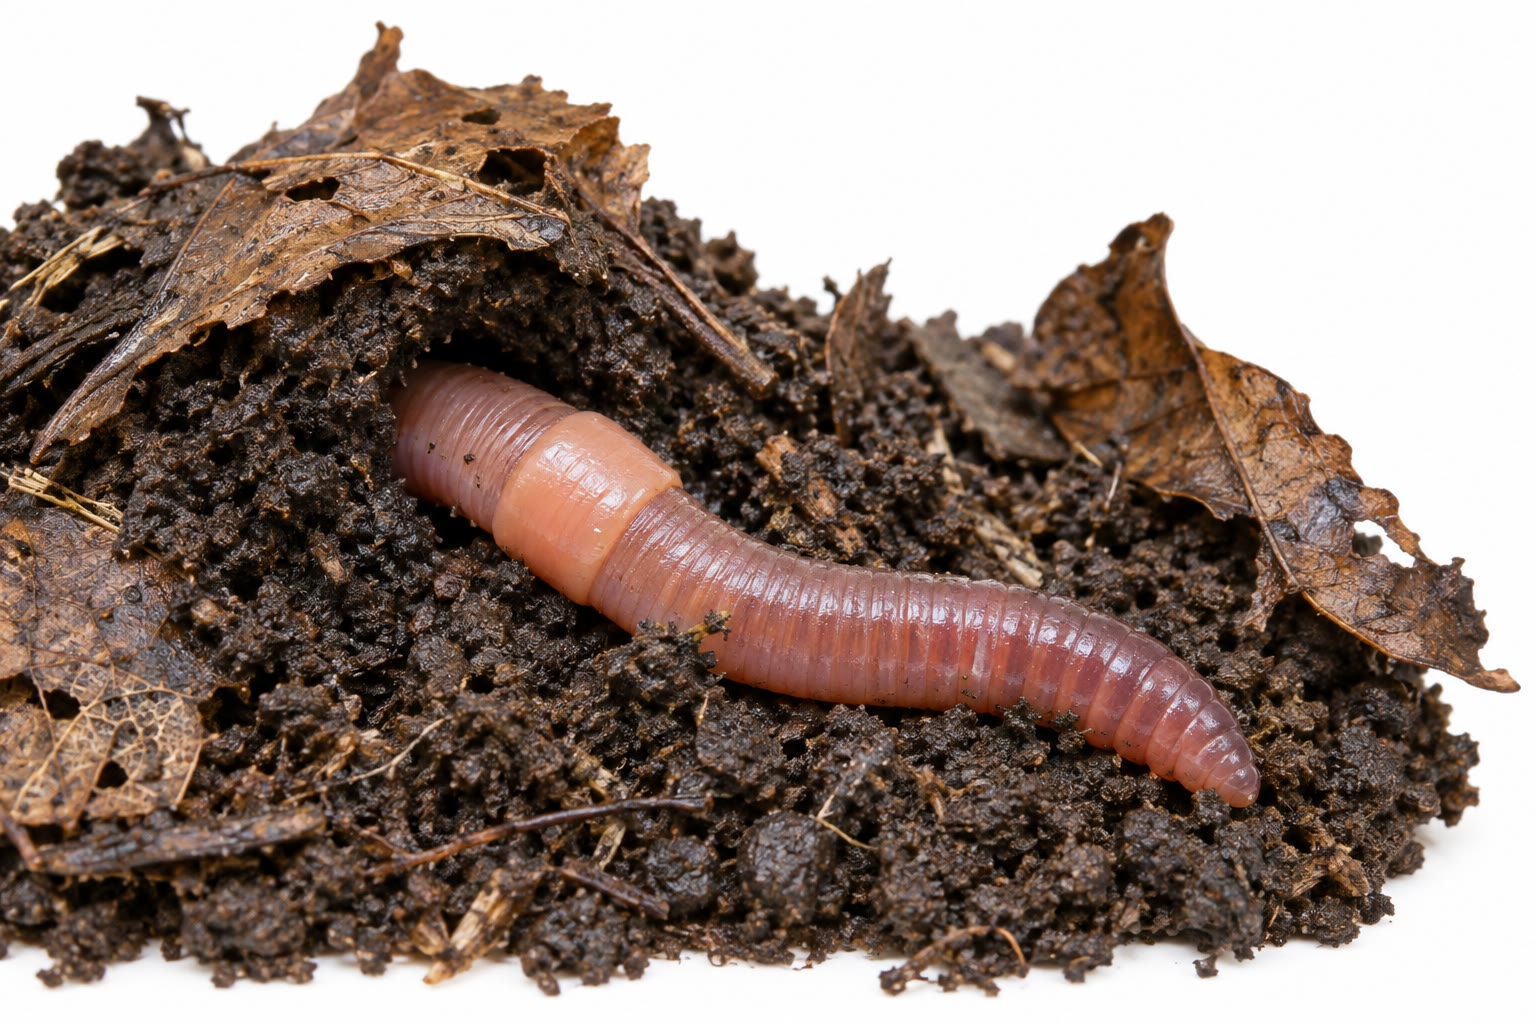
\includegraphics[width=0.42\linewidth]{images/book4/ai/b4-26-earthworm.jpg}\hspace{0.025\linewidth}
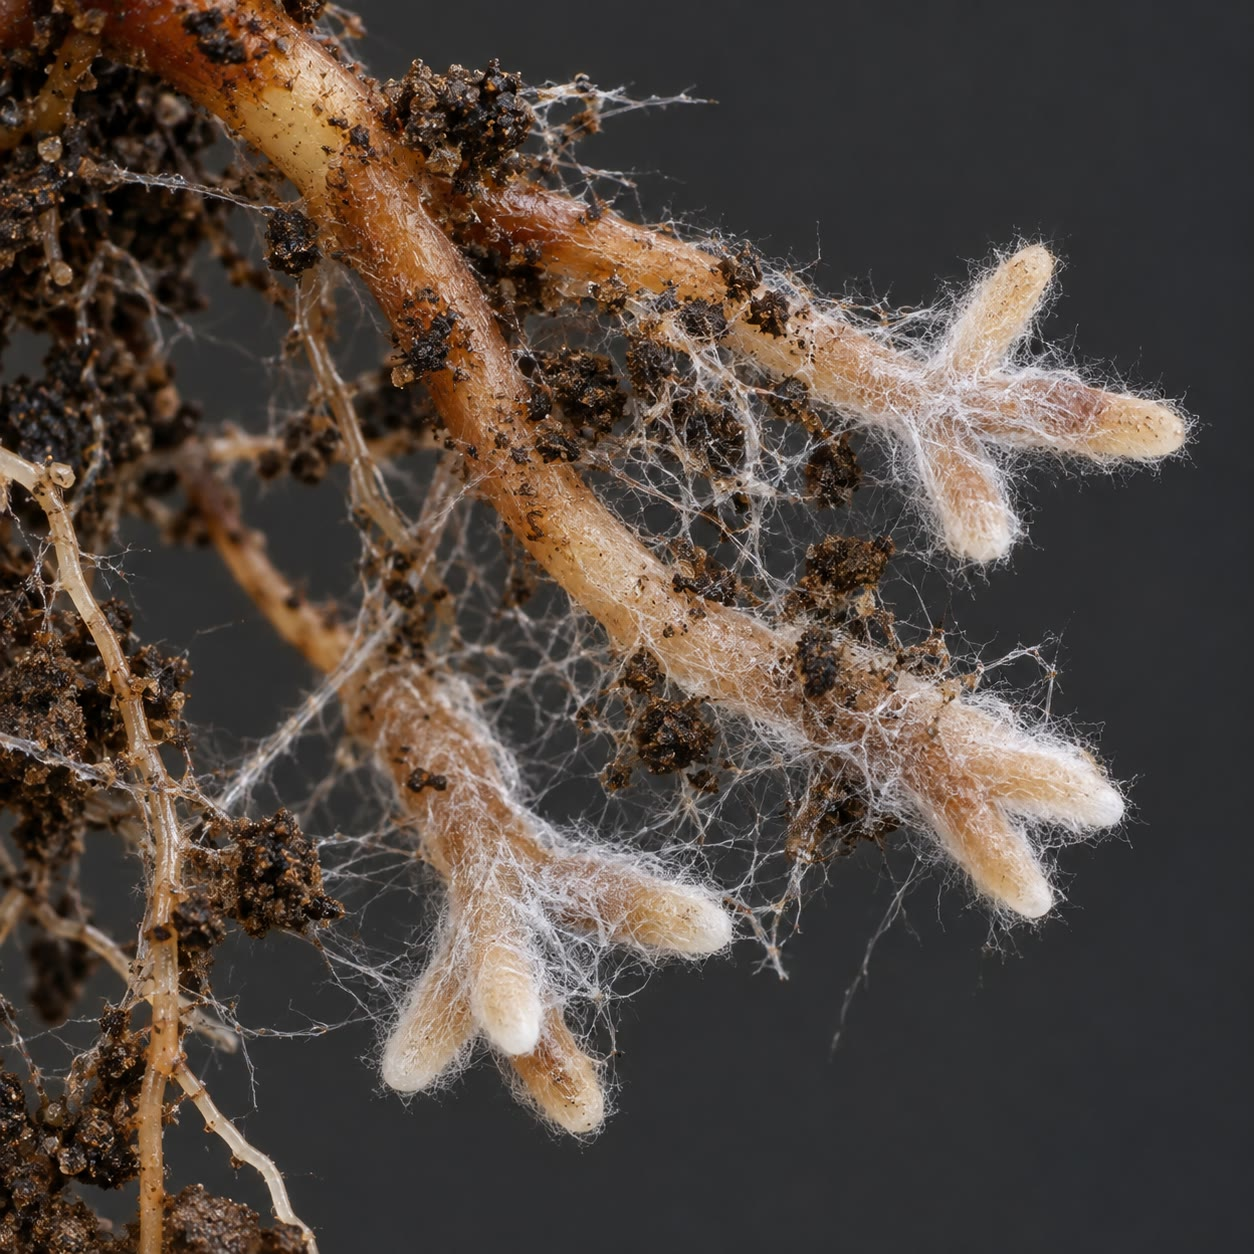
\includegraphics[width=0.28\linewidth]{images/book4/ai/b4-26-mycorrhiza.jpg}

{\small O \omterm{def:b2:living-soil:soil}{solo} e dois de seus artífices. À esquerda: um perfil num
barranco, com a camada superficial escura passando gradualmente à rocha
alterada clara. No meio: uma minhoca em sua galeria. À direita: uma raiz
com seu manto ectomicorrízico e as hifas que a prolongam no \omterm{def:b2:living-soil:soil}{solo}.}
\end{omfigure}

\section{Decomposição}

\begin{theorem}[A decomposição da serapilheira e a razão carbono/nitrogênio]\label{thm:b2:living-soil:decay}
\index{decomposição}\index{decomposição da serapilheira}\index{razão C:N}\index{mineralização}\index{imobilização}
A serapilheira se decompõe a uma taxa proporcional ao que resta,
$\mathrm{d}L/\mathrm{d}t = -kL$, logo $L = L_0 e^{-kt}$, com uma
\emph{constante de decomposição} $k$ de cerca de 1 por ano para gramíneas
e folhas caducas numa floresta temperada, $0.3$ para acículas de
coníferas, várias por ano nos trópicos úmidos e $0.05$ na tundra;
uma entrada constante $I$ por ano forma uma camada de serapilheira de
$I/k$. A decomposição é controlada pela temperatura, pela umidade e pela
\emph{qualidade} da serapilheira: teor de nitrogênio, teor de lignina e
razão entre carbono e nitrogênio. Os micróbios têm $\mathrm{C:N} \approx 8$
e retêm cerca de \qty{40}{\%} do carbono que comem, de modo que precisam
de um nitrogênio para cada $8/0.4 = 20$ carbonos de alimento: a
serapilheira com $\mathrm{C:N}$
abaixo de cerca de 25 libera amônio ao se decompor
(\emph{mineralização}), ao passo que a serapilheira acima desse valor ---
a palha a 80, a \omterm{def:b2:plant-meristems:wood}{madeira} a 400 --- faz os micróbios retirarem nitrogênio
do \omterm{def:b2:living-soil:soil}{solo} (\emph{imobilização}), privando as plantas até que o carbono
tenha sido respirado e a razão tenha caído. É por isso que a palha
fresca incorporada ao \omterm{def:b2:living-soil:soil}{solo} prejudica uma cultura, que os resíduos de
leguminosas a alimentam, e que uma composteira precisa de ambos.
\end{theorem}
\begin{proof}
Para a razão: os micróbios que comem serapilheira com $c$ carbonos por
nitrogênio assimilam $0.4c$ carbonos e, para construir biomassa com
$\mathrm{C:N} = 8$, precisam de $0.4c/8 = c/20$ nitrogênios; a
serapilheira fornece 1. Se $c < 20$, sobra nitrogênio, liberado como
amônio; se $c > 20$, há um déficit retirado do \omterm{def:b2:living-soil:soil}{solo}. O limiar de 25 na
prática reflete uma eficiência de retenção um pouco abaixo de 0.4. Para
a camada de serapilheira: $\mathrm{d}L/\mathrm{d}t = I - kL$
tem o \omterm{def:b2:biogeochemical-cycles:reservoir}{estado estacionário} $I/k$, atingido com a constante de tempo $1/k$;
o \omterm{def:b2:biogeochemical-cycles:reservoir}{tempo de residência} da serapilheira é $1/k$, um ano numa floresta de
faias e vinte na tundra.
\end{proof}
\begin{proof}[Evidências]
Os experimentos com sacos de serapilheira --- massas conhecidas de folhas
em sacos de tela, enterrados e pesados a intervalos --- deram a lei
exponencial e suas constantes em todos os biomas (Olson, 1963), e
mostraram, com diferentes tamanhos de malha, que excluir os animais do
\omterm{def:b2:living-soil:soil}{solo} reduz a taxa à metade: os micróbios fazem a química, mas os animais
ditam o ritmo. De um lado a outro de um continente, a mesma folha se
decompõe em um ano na Geórgia e em oito no Alasca, proporcionalmente à
evapotranspiração real, o produto do calor pela água.
\end{proof}

\begin{omfigure}
\begin{tikzpicture}
\begin{axis}[
  width=0.72\linewidth, height=5.6cm,
  axis x line=bottom, axis y line=left,
  xmin=0, xmax=6, ymin=0, ymax=105,
  xlabel={anos}, ylabel={massa de serapilheira restante (\%)},
  xlabel style={font=\small, at={(axis description cs:0.5,-0.13)}, anchor=north},
  ylabel style={font=\small},
  tick label style={font=\small},
  legend style={font=\scriptsize, at={(0.5,-0.3)}, anchor=north, draw=none, legend columns=2},
  clip=false,
]
\addplot[very thick, omDef, domain=0:6, samples=60] {100*exp(-2*x)};
\addlegendentry{folha de floresta tropical, $k = 2$}
\addplot[very thick, omThm, domain=0:6, samples=60] {100*exp(-1*x)};
\addlegendentry{folha de faia, $k = 1$}
\addplot[very thick, omProp, domain=0:6, samples=60] {100*exp(-0.3*x)};
\addlegendentry{acícula de espruce, $k = 0.3$}
\addplot[very thick, gray, domain=0:6, samples=60] {100*exp(-0.05*x)};
\addlegendentry{musgo da tundra, $k = 0.05$}
\end{axis}
\end{tikzpicture}

{\small Decomposição exponencial da serapilheira. Metade de uma folha de
faia desaparece em oito meses; metade de um \omterm{def:b2:plant-life-cycles:moss}{musgo} da tundra, em catorze
anos; o resíduo que nem micróbio nem animal consegue terminar se torna
\omterm{def:b2:living-soil:soil}{húmus}.}
\end{omfigure}

\begin{proposition}[O húmus e o estoque de carbono do solo]\label{prop:b2:living-soil:humus}
\index{húmus}\index{carbono orgânico do solo}\index{respiração do solo}
Alguns por cento do carbono da serapilheira escapam da oxidação completa
e se tornam \emph{\omterm{def:b2:living-soil:soil}{húmus}}: uma mistura escura e amorfa de resíduos
microbianos, lignina alterada e compostos vegetais, ligada à argila e ao
ferro e presa nos agregados, que se decompõe com \omterm{def:b2:biogeochemical-cycles:reservoir}{tempos de residência} de
décadas a milênios. É no \omterm{def:b2:living-soil:soil}{húmus} que vive a fertilidade do \omterm{def:b2:living-soil:soil}{solo}
--- a maior parte de seu nitrogênio e de sua troca catiônica, metade de
sua retenção de água --- e ele é o maior estoque de carbono orgânico em
terra, \qty{1700}{GtC} no primeiro metro, o dobro do da atmosfera. Seu
balanço é entrada menos decomposição, $\mathrm{d}H/\mathrm{d}t = I_h - k_hH$:
com $k_h \approx 0.02$ por ano, um \omterm{def:b2:living-soil:soil}{solo} contém cinquenta anos de entrada,
e qualquer mudança --- a aração, que quebra os agregados e areja o
\omterm{def:b2:living-soil:soil}{húmus}; a drenagem de uma turfeira, que deixa entrar o oxigênio; o
aquecimento, que eleva $k_h$ --- aparece como uma perda que continua
por décadas. Os \omterm{def:b2:living-soil:soil}{solos} cultivados do mundo perderam de um terço à metade
de seu \omterm{def:b2:living-soil:soil}{húmus} desde que foram lavrados pela primeira vez, cerca de
\qty{100}{GtC}, e um aquecimento de \qty{3}{\celsius} aumentaria em um
terço a decomposição do restante: os \omterm{def:b2:living-soil:soil}{solos} são a maior incerteza do
balanço de carbono do \cref{ch:b2:global-change}.
\end{proposition}

\section{Parcerias subterrâneas}

\begin{proposition}[Micorrizas e rizóbios]\label{prop:b2:living-soil:symbiosis}
\index{micorriza}\index{rizóbio}\index{nódulo radicular}\index{nitrogenase}\index{leghemoglobina}
Nove espécies de plantas em cada dez têm as raízes colonizadas por
fungos numa \emph{micorriza}: a planta dá açúcar (de um décimo a um
quinto de seus fotoassimilados) e o fungo dá fosfato, nitrogênio, água e
zinco, que suas hifas, cem vezes mais finas que uma raiz e com cem vezes
o comprimento dela por unidade de carbono, coletam num volume de \omterm{def:b2:living-soil:soil}{solo} que
a raiz não alcança --- o fosfato em particular, que se difunde tão
lentamente no \omterm{def:b2:living-soil:soil}{solo} que uma raiz esgota seu milímetro de vizinhança em
poucos dias. As micorrizas \emph{arbusculares}, o tipo mais antigo,
penetram nas células da raiz e se ramificam em arbúsculos, onde ocorre a
troca; as \emph{ectomicorrizas} das árvores florestais envolvem a ponta
da raiz e crescem entre suas células. As leguminosas vão além: os
rizóbios, atraídos pelos flavonoides da raiz, entram por um \omterm{prop:b2:plant-meristems:ram}{pelo
radicular}, e a raiz constrói em torno deles um \emph{nódulo} no qual as
bactérias, como \emph{bacteroides}, fixam nitrogênio com a nitrogenase
--- uma enzima tão sensível ao oxigênio que o nódulo precisa ser mantido
quase anóxico pela \emph{leghemoglobina}, uma hemoglobina produzida pela
planta, que dá ao nódulo sua cor rosada e entrega oxigênio aos
bacteroides numa concentração baixa demais para envenenar a enzima. Cada
parceiro fiscaliza o outro: uma planta corta o açúcar dos nódulos que
não fixam nada, e um fungo que entrega menos fosfato recebe menos
carbono.
\end{proposition}
\begin{proof}[Evidências]
Kiers e colaboradores (2011) cultivaram uma planta com dois fungos
parceiros num sistema radicular dividido e ofereceram fosfato a um só
lado: a planta destinou mais carbono ao fungo que fornecia mais fosfato,
e o fungo destinou mais fosfato a uma raiz que dava mais carbono ---
recompensas recíprocas medidas com isótopos. Para os rizóbios, nódulos
experimentalmente impedidos de fixar (substituindo-se o ar por argônio e
oxigênio) receberam menos oxigênio e cresceram menos que nódulos da mesma
planta que podiam fixar: a planta pune os trapaceiros. A marcação com
nitrogênio-15 mostra que uma pastagem de trevo e gramínea transfere um
terço do nitrogênio fixado pelo trevo para a gramínea em uma estação,
através do \omterm{def:b2:living-soil:soil}{solo} e das redes de fungos compartilhadas.
\end{proof}

\begin{omfigure}
\begin{tikzpicture}[every node/.style={font=\scriptsize}, >=stealth]
  % root cross-section
  \fill[omThm!15] (0,0) circle (1.5); \draw[thick] (0,0) circle (1.5);
  \fill[omThm!30] (0,0) circle (0.5); \draw[thick] (0,0) circle (0.5);
  \node at (0,0) {cilindro central};
  \node at (0,1.05) {córtex};
  % arbuscules in cortex cells
  \foreach \a in {30,150,270} { \draw[omDef, thick] ({1.0*cos(\a)},{1.0*sin(\a)}) -- ++({0.25*cos(\a+60)},{0.25*sin(\a+60)}) -- ++({0.2*cos(\a-40)},{0.2*sin(\a-40)}); \draw[omDef, thick] ({1.0*cos(\a)},{1.0*sin(\a)}) -- ++({0.25*cos(\a-60)},{0.25*sin(\a-60)}); }
  % hyphae out
  \foreach \a in {20,80,150,210,340} { \draw[omDef, thick] ({1.5*cos(\a)},{1.5*sin(\a)}) .. controls ({2.2*cos(\a+10)},{2.2*sin(\a+10)}) .. ({2.7*cos(\a-5)},{2.7*sin(\a-5)}); }
  \draw[omDef, thick] ({1.5*cos(150)},{1.5*sin(150)}) -- ({1.0*cos(150)},{1.0*sin(150)});
  \node[omDef, anchor=west, align=left] at (2.9,1.4) {hifas: \qty{3}{\micro m} de largura,\\ metros por centímetro de raiz};
  \node[omDef, anchor=west] at (2.9,0.1) {arbúsculo numa célula do córtex};
  \draw[omDef] (2.85,0.1) -- (1.2,0.5);
  \node[anchor=north, align=center] at (0,-1.6) {raiz, \qty{0.3}{mm} de diâmetro};
  \draw[->, thick, omThm] (-1.2,-2.4) -- (1.2,-2.4) node[right] {açúcar para o fungo, \qtyrange{10}{20}{\%} dos fotoassimilados};
  \draw[<-, thick, omDef] (-1.2,-2.9) -- (1.2,-2.9) node[right] {fosfato, amônio, água e zinco para a planta};
  % nodule
  \begin{scope}[xshift=9.3cm]
    \draw[thick, brown!60!black] (-0.3,2.4) -- (-0.1,-0.6);
    \draw[thick, brown!60!black] (-0.1,0.3) -- (1.6,0.1);
    \fill[pink!60!red!40] (1.5,0.2) circle (0.9); \draw[thick] (1.5,0.2) circle (0.9);
    \fill[pink!80!red!60] (1.5,0.2) circle (0.55);
    \foreach \p in {(1.3,0.3),(1.6,0.0),(1.5,0.45),(1.7,0.3),(1.35,0.05)} \fill[omDef!70!black] \p ellipse (0.08 and 0.05);
    \node[anchor=north, align=center] at (1.5,-0.8) {nódulo: bacteroides em\\ células vegetais, rosado pela\\ leghemoglobina; oxigênio a \qty{10}{nM},\\ a nitrogenase funciona\\ e as células respiram};
    \node[anchor=south, align=center] at (-0.2,2.45) {raiz de leguminosa};
  \end{scope}
\end{tikzpicture}

{\small Duas barganhas. À esquerda: uma micorriza arbuscular, com o
açúcar saindo e o fosfato entrando pelos arbúsculos dentro das células
do córtex. À direita: um nódulo de leguminosa, onde a hemoglobina da
própria planta mantém o oxigênio baixo o bastante para a nitrogenase e
alto o bastante para a respiração.}
\end{omfigure}

\section{Perder o solo}

\begin{proposition}[Erosão, sal e o balanço de um solo]\label{prop:b2:living-soil:erosion}
\index{erosão do solo}\index{salinização}\index{desertificação}
O \omterm{def:b2:living-soil:soil}{solo} se forma a \qtyrange{0.05}{0.5}{mm} por ano e, sob vegetação
natural, sofre erosão mais ou menos no mesmo ritmo. Uma terra nua e
arada numa encosta perde \qtyrange{1}{10}{mm} por ano pela água e pelo
vento --- \qtyrange{10}{100}{t/ha} ---, de dez a cem vezes a taxa de
formação: um \omterm{def:b2:living-soil:soil}{solo} construído em dez mil anos é removido em um século, e
com ele o \omterm{def:b2:living-soil:soil}{húmus} e os nutrientes do horizonte A, a única parte que
importa. As culturas de cobertura, os terraços, a aração em curvas de
nível e o plantio direto, que deixa os resíduos na superfície e os
agregados intactos, trazem a perda de volta para perto da taxa de
formação. A irrigação em climas secos traz o fracasso oposto: a água
evapora e deixa seus sais, uma tonelada por hectare por ano a partir de
uma água apenas ligeiramente salina, até que o potencial osmótico da
solução do \omterm{def:b2:living-soil:soil}{solo} (\cref{ch:b2:plant-plasticity}) fique mais baixo do que
as raízes conseguem vencer --- a \emph{salinização}, que tirou de uso os
campos da Suméria há quatro mil anos e hoje afeta um quinto das terras
irrigadas. O estado de um \omterm{def:b2:living-soil:soil}{solo} é um balanço: \omterm{def:b2:living-soil:soil}{húmus} que entra contra
\omterm{def:b2:living-soil:soil}{húmus} que sai, formação contra erosão, sal que entra contra sal drenado;
cada um tem um \omterm{def:b2:biogeochemical-cycles:reservoir}{tempo de residência} e cada um, uma vez negativo, é lento
para se reverter.
\end{proposition}

\section{Exercícios}

\begin{exercise}[$\star$]\label{exo:b2:living-soil:1}
Nomeie os horizontes de um perfil de \omterm{def:b2:living-soil:soil}{solo}, da superfície para baixo, e
diga o que acontece em cada um.
\end{exercise}

\begin{exercise}[$\star$]\label{exo:b2:living-soil:2}
Explique o que é a \omterm{prop:b2:living-soil:cec}{capacidade de troca catiônica}, por que um \omterm{def:b2:living-soil:soil}{solo}
arenoso tem pouca, e o que faz ao \omterm{def:b2:living-soil:soil}{solo} um agricultor que aplica calcário
num \omterm{def:b2:living-soil:soil}{solo} ácido.
\end{exercise}

\begin{exercise}[$\star$]\label{exo:b2:living-soil:3}
Liste os principais grupos da \omterm{prop:b2:living-soil:community}{teia alimentar do solo}, dos decompositores
aos predadores de topo, com um organismo de cada, e diga o que os
pastadores de bactérias fazem pelas plantas.
\end{exercise}

\begin{exercise}[$\star$]\label{exo:b2:living-soil:4}
Distinga as micorrizas arbusculares das ectomicorrizas, e diga o que
cada parceiro dá e recebe.
\end{exercise}

\begin{exercise}[$\star\star$]\label{exo:b2:living-soil:5}
Uma floresta de faias deixa cair \qty{4}{t/ha} de folhas por ano, e sua
serapilheira se decompõe com $k = 0.8$ por ano. Calcule a massa de
serapilheira em \omterm{def:b2:biogeochemical-cycles:reservoir}{estado estacionário}, o \omterm{def:b2:biogeochemical-cycles:reservoir}{tempo de residência} da
serapilheira e o tempo para que a queda de um ano perca \qty{90}{\%} de
sua massa.
\end{exercise}

\begin{exercise}[$\star\star$]\label{exo:b2:living-soil:6}
A palha de trigo tem $\mathrm{C:N} = 80$ e os resíduos de trevo, $15$.
Para cada um, calcule o nitrogênio de que os micróbios precisam por
\qty{100}{kg} de carbono consumido (retenção de 0.4, $\mathrm{C:N} = 8$
nos micróbios) e se o resíduo mineraliza ou imobiliza, e quanto.
\end{exercise}

\begin{exercise}[$\star\star$]\label{exo:b2:living-soil:7}
Um hectare de pastagem contém \qty{2}{t} de minhocas, cada uma das quais
processa dez vezes sua massa em \omterm{def:b2:living-soil:soil}{solo} por ano. Calcule o \omterm{def:b2:living-soil:soil}{solo} que passa
pelas minhocas por ano e o tempo para que os \qty{20}{cm} superficiais
(densidade aparente de \qty{1.3}{t/m^3}) passem por elas uma vez.
Compare com o número de Darwin.
\end{exercise}

\begin{exercise}[$\star\star$]\label{exo:b2:living-soil:8}
Um grama de \omterm{def:b2:living-soil:soil}{solo} contém $10^{9}$ bactérias de massa \qty{e-12}{g} cada,
e \qty{100}{m} de hifas de diâmetro \qty{4}{\micro m} e densidade
\qty{1.1}{g/cm^3}. Calcule a biomassa bacteriana e fúngica por grama e
por hectare (\qty{20}{cm} superficiais, \qty{1.3}{t/m^3}).
\end{exercise}

\begin{exercise}[$\star\star$]\label{exo:b2:living-soil:9}
O \omterm{def:b2:living-soil:soil}{húmus} de um \omterm{def:b2:living-soil:soil}{solo} se decompõe com $k_h = 0.02$ por ano e recebe
\qty{1.5}{t/ha} de carbono por ano. Calcule o carbono do \omterm{def:b2:living-soil:soil}{húmus} em \omterm{def:b2:biogeochemical-cycles:reservoir}{estado
estacionário}. O campo é arado e $k_h$ dobra: calcule o novo \omterm{def:b2:biogeochemical-cycles:reservoir}{estado
estacionário}, o carbono perdido e o tempo para perder metade dele.
\end{exercise}

\begin{exercise}[$\star\star\star$]\label{exo:b2:living-soil:10}
O fosfato se difunde no \omterm{def:b2:living-soil:soil}{solo} com $D \approx \qty{e-13}{m^2/s}$.
Calcule a distância que ele percorre numa estação de crescimento de
\num{100} dias ($x \approx \sqrt{2Dt}$) e compare com o espaçamento das
raízes (\qty{1}{cm}) e das hifas (\qty{0.1}{mm}). O que isso diz sobre
por que as micorrizas importam para o fósforo, e menos para o nitrato
($D \approx \qty{e-10}{m^2/s}$)?
\end{exercise}

\begin{exercise}[$\star\star\star$]\label{exo:b2:living-soil:11}
Uma encosta perde \qty{20}{t/ha} de \omterm{def:b2:living-soil:soil}{solo} por ano por erosão enquanto
forma \qty{1}{t/ha}; o horizonte A tem \qty{25}{cm} de espessura, com
\qty{1.3}{t/m^3}, e contém \qty{3}{\%} de carbono. Calcule a massa do
horizonte A, seu tempo de vida nesse ritmo e o carbono perdido por ano.
Sob plantio direto, a perda cai para \qty{2}{t/ha}: recalcule o tempo de
vida.
\end{exercise}

\begin{exercise}[$\star\star\star$]\label{exo:b2:living-soil:12}
``O \omterm{def:b2:living-soil:soil}{solo} é o organismo mais lento da propriedade.'' Discuta com os
\omterm{def:b2:biogeochemical-cycles:reservoir}{tempos de residência} da serapilheira, do \omterm{def:b2:living-soil:soil}{húmus}, do \omterm{def:b2:living-soil:soil}{solo} mineral e do sal,
e diga quais mudanças um agricultor pode ver ao longo de uma carreira e
quais não.
\end{exercise}

\section{Problema: Um hectare de solo}

\begin{problem}[{Problema de fim de semana --- um hectare de solo arável
auditado: sua massa viva contada, sua serapilheira e seu húmus
acompanhados por meio de seus balanços exponenciais, o nitrogênio
liberado por um resíduo de leguminosa calculado em relação à necessidade
de uma cultura, e os balanços de erosão e de carbono de dois sistemas de
manejo comparados, terminando com o estoque de carbono do solo, seu
tempo de vida sob aração e o nitrogênio que uma leguminosa fornece}]
\label{pb:b2:living-soil:1}
O hectare: horizonte A de \qty{25}{cm} de espessura, densidade aparente
de \qty{1.3}{t/m^3}, \qty{2.5}{\%} de carbono orgânico; decomposição do
\omterm{def:b2:living-soil:soil}{húmus} $k_h =
0.025$ por ano sob aração, $0.015$ sob plantio direto; entrada de carbono
no \omterm{def:b2:living-soil:soil}{húmus} de \qty{1.2}{t/ha} por ano nos dois casos. Serapilheira: uma
cultura de cobertura de trevo deixa \qty{5}{t/ha} de matéria seca com
\qty{45}{\%} de carbono e \qty{3}{\%} de nitrogênio, que se decompõe com
$k = 2$ por ano. Erosão: \qty{15}{t/ha} por ano com aração,
\qty{1.5}{t/ha} com plantio direto; formação de \qty{0.5}{t/ha}.

\medskip
\noindent\textbf{Parte I --- O estoque.}
\begin{enumerate}
  \item Calcule a massa do horizonte A e seu carbono orgânico.
  \item Calcule a massa de nitrogênio no \omterm{def:b2:living-soil:soil}{húmus} se sua
        $\mathrm{C:N}$ for 12.
  \item O \omterm{def:b2:living-soil:soil}{solo} contém $10^{9}$ bactérias por grama, de \qty{e-12}{g}
        cada, e \qty{200}{m} de hifas por grama, de \qty{4}{\micro m}
        de diâmetro e densidade 1.1. Calcule a biomassa microbiana por
        hectare.
  \item Acrescente \qty{1.5}{t/ha} de minhocas e \qty{0.2}{t/ha} de
        outros animais, e dê a massa viva total por hectare.
        Que fração do carbono do \omterm{def:b2:living-soil:soil}{húmus} ela representa?
  \item Os micróbios renovam sua biomassa duas vezes por ano e
        respiram \qty{60}{\%} do que comem. Estime o carbono que
        consomem por ano e o $\mathrm{CO_2}$ respirado.
  \item Compare com a produção primária líquida da cultura, de cerca de
        \qty{5}{t/ha} de carbono, e comente.
\end{enumerate}

\medskip
\noindent\textbf{Parte II --- O resíduo de trevo.}
\begin{enumerate}[resume]
  \item Calcule o carbono e o nitrogênio do resíduo e sua
        $\mathrm{C:N}$.
  \item Com $\mathrm{C:N} = 8$ nos micróbios e retenção de $0.4$, o
        resíduo mineraliza ou imobiliza nitrogênio? Calcule o
        nitrogênio líquido liberado quando todo o resíduo se decompõe.
  \item Com $k = 2$, que fração do resíduo se decompôs após
        3 meses? E após um ano?
  \item Calcule o nitrogênio liberado nos primeiros 3 meses.
  \item Uma cultura de trigo absorve \qty{150}{kg} de nitrogênio por hectare,
        a maior parte nos dois meses após a semeadura. Comente o
        momento.
  \item A mesma massa de palha de trigo ($\mathrm{C:N} = 80$) é
        incorporada em seu lugar. Calcule o nitrogênio imobilizado e
        diga o que o agricultor deve fazer.
\end{enumerate}

\medskip
\noindent\textbf{Parte III --- O \omterm{def:b2:living-soil:soil}{húmus}.}
\begin{enumerate}[resume]
  \item Calcule o carbono do \omterm{def:b2:living-soil:soil}{húmus} em \omterm{def:b2:biogeochemical-cycles:reservoir}{estado estacionário} sob aração e
        sob plantio direto.
  \item O campo, no \omterm{def:b2:biogeochemical-cycles:reservoir}{estado estacionário} sob aração, é convertido ao
        plantio direto. Escreva $H(t)$ e calcule o carbono ganho após
        10 e 50 anos.
  \item Calcule a taxa de ganho no primeiro ano, em toneladas de
        carbono por hectare e em toneladas de $\mathrm{CO_2}$.
  \item Se os \qty{1.5e9}{ha} de terras cultivadas do mundo fizessem o
        mesmo, qual seria o sumidouro do primeiro ano, diante de emissões
        fósseis de \qty{10}{GtC}? E no quinquagésimo ano?
  \item Por que o sumidouro é temporário e reversível?
  \item Um aquecimento de \qty{3}{\celsius} eleva $k_h$ em um terço.
        Calcule o novo \omterm{def:b2:biogeochemical-cycles:reservoir}{estado estacionário} sob plantio direto e o carbono perdido.
\end{enumerate}

\medskip
\noindent\textbf{Parte IV --- A erosão.}
\begin{enumerate}[resume]
  \item Calcule a perda líquida de \omterm{def:b2:living-soil:soil}{solo} por ano em cada sistema.
  \item Calcule o tempo de vida do horizonte A em cada um.
  \item Calcule o carbono e o nitrogênio levados por ano pela
        erosão sob aração.
  \item Compare a perda de carbono por erosão com a perda por
        decomposição do \omterm{def:b2:living-soil:soil}{húmus} no \omterm{def:b2:biogeochemical-cycles:reservoir}{estado estacionário} sob aração.
  \item O \omterm{def:b2:living-soil:soil}{solo} erodido é depositado a jusante. Seu carbono é
        perdido para a atmosfera? Discuta.
  \item Dê os \omterm{def:b2:biogeochemical-cycles:reservoir}{tempos de residência} da serapilheira, do \omterm{def:b2:living-soil:soil}{húmus} e do \omterm{def:b2:living-soil:soil}{solo}
        mineral neste hectare.
  \item Enuncie o resultado: o estoque de carbono do horizonte A, seu
        tempo de vida sob aração e sob plantio direto, e o
        nitrogênio que o resíduo de trevo fornece.
\end{enumerate}
\end{problem}
